\begin{tcolorbox}[title={Inhalt}]
\begin{itemize} 
    \item Was sind Neuronen
    \item Arten von Neuronen
    \item Funktionsweise
    \item Aktivierungsfunktion
    \item Schichtenmodell
\end{itemize} 
\end{tcolorbox}
\subsection{Was sind Neuronen?}\label{sec:neuronen:was_sind_neuronen}  
Das menschliche Nervensystem besteht aus Neuronen, welche mit Axonen oder Dendriten verknüpft sind. Diese Verbindungen werden auch Synapsen genannt. Die variable Stärke der Synapsen
ermöglichen das Lernen. Dieser biologische Mechanismus wird durch neurale Netze simuliert.\\

\begin{figure}[H]
\begin{subfigure}{0.6\textwidth}
    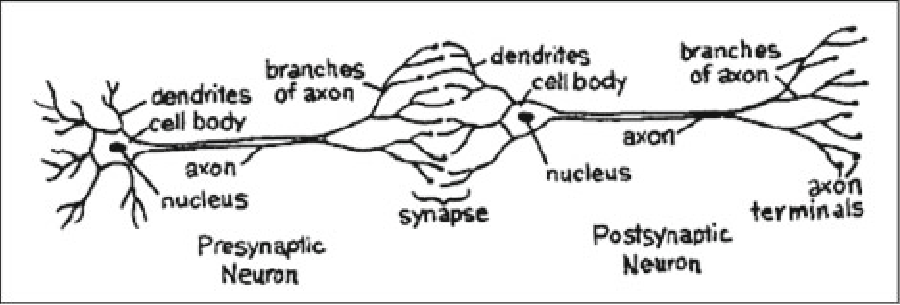
\includegraphics[width=\textwidth]{Sources/01-01_synapse.png}
    \label{Synapse}
    \caption{Synapse}
\end{subfigure}
\begin{subfigure}{0.25\textwidth}
    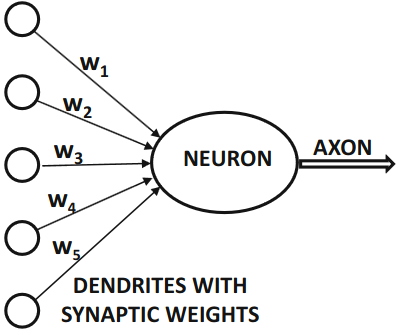
\includegraphics[width=\textwidth]{Sources/01-02_neuron.png}
    \label{Neuron}
    \caption{Neuron}
\end{subfigure}
\caption{Neural Networks and Deep Learning A Textbook, Charu C. Aggarwal
}
\end{figure}

Eines neuronales Netz besteht aus mindestens einem Neuron. Neuronen sind essentielle Bestandteile von neuralen Netzen. Sie nehmen Eingabedaten entgegen und wandeln diese 
in Ausgabedaten um. Neben den Eingabedaten werden auch Weight-Parameter übergeben, welche die zu berechnenden Werte beinflussen. Das eigenliche \enquote{Lernen} erfolgt durch diesen 
Einfluss.
\subsection{Arten von Neuronen}\label{subsec:neuronen:arten_von_neuronen}
  TEXT FOLGT... 